\input{../latexSetup}

\usepackage{tikz}
\usetikzlibrary{arrows.meta}

\lhead{\Large 33-211}
\chead{\Large Physics 3 : Modern Essentials}
\rhead{\Large Lecture 2}

\begin{document}
\thispagestyle{fancy}

\begin{center}
  {\huge \textbf{Classical Physics --- ``Newtonian'' (Reminder)}}
\end{center}

% ============================================================
\section*{The Classical Picture}

The world is described by \emph{objects} (particles) moving in space and time.

(Intro. discussion about Coordinate changes to solve problems. eg: pouring drinks in airplanes)

\subsection*{Spacetime Diagrams (1D)}

A \textbf{spacetime diagram} plots position $x$ (horizontal) vs.\ time $t$ (vertical).
Each particle traces a \emph{worldline}.

\begin{center}
\begin{tikzpicture}[scale=1.5, >=Stealth]
  % Axes
  \draw[->] (-0.3,0) -- (3.0,0) node[right] {$x$};
  \draw[->] (0,-0.2) -- (0,3.2) node[above] {$t$};

  % v=0: vertical red line
  \draw[red, thick] (0.5,0) -- (0.5,3);
  \node[red, left, font=\small] at (0.5,2.8) {$v=0$};

  % v>0: tilted green line, with labels
  \draw[green!60!black, thick] (0.9,0) -- (2.1,3);
  \node[green!60!black, right, align=left, font=\small] at (1.25,1.2)
    {$v>0$ \\ $p = mv$ \\ $E = \tfrac{1}{2}mv^2$};

  % Forced particle: blue with a kink (force applied at midpoint)
  \draw[blue, thick] (1.9,0) -- (2.2,1.4);
  \fill[blue] (2.2,1.4) circle (1.5pt);
  \draw[blue, thick] (2.2,1.4) -- (2.7,3);

  % Annotation: forces curve the worldlines
  \node[align=left, font=\small] at (4.6,2.8)
    {Forces specify how \\ the lines curve};
  \draw[->, thin] (3.5,2.5) -- (2.5,2.0);
  \node[font=\normalsize] at (4.5,1.8)
    {$\vec{F} = \dfrac{d\vec{p}}{dt}$};
\end{tikzpicture}
\end{center}

\begin{itemize}
  \item Particles with \textbf{no forces} move in \textbf{straight lines}.
  \item Forces specify how worldlines \emph{curve}: $\vec{F} = \dfrac{d\vec{p}}{dt}$.
\end{itemize}

\subsubsection*{Same Situation in a Different Reference Frame $F'$ (moving with velocity $v$)}

\begin{center}
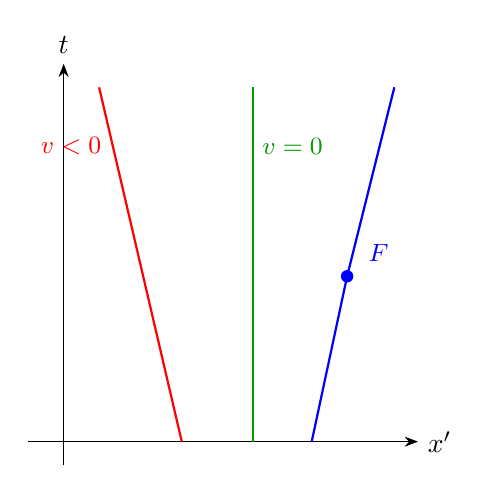
\begin{tikzpicture}[scale=1.5, >=Stealth]
  \draw[->] (-0.3,0) -- (3.0,0) node[right] {$x'$};
  \draw[->] (0,-0.2) -- (0,3.2) node[above] {$t$};

  % Previously v=0, now appears to move left: red, tilted left
  \draw[red, thick] (1.0,0) -- (0.3,3);
  \node[red, left, font=\small] at (0.4,2.5) {$v<0$};

  % Previously v>0, now appears stationary: green, vertical
  \draw[green!60!black, thick] (1.6,0) -- (1.6,3);
  \node[green!60!black, right, font=\small] at (1.6,2.5) {$v=0$};

  % Forced particle still has a kink
  \draw[blue, thick] (2.1,0) -- (2.4,1.4);
  \fill[blue] (2.4,1.4) circle (1.5pt);
  \draw[blue, thick] (2.4,1.4) -- (2.8,3);
  \node[blue, right, font=\small] at (2.5,1.6) {$F$};
\end{tikzpicture}
\end{center}

\textbf{Nomenclature:} Note that $\vec{p}$ and $E$ are \underline{not invariant} under a frame change.
\underline{Masses are invariant}.

% ============================================================
\section*{Elastic Collision Example}

Two identical particles collide elastically.  In the CM frame, total momentum is zero.

\begin{center}
\begin{tikzpicture}[scale=1.1, >=Stealth]
  % Collision point
  \filldraw (0,0) circle (2pt);
  \draw[thin, gray] (-2.5,0) -- (2.5,0);
  \draw[thin, gray] (0,-2) -- (0,2);
  \node[gray, right, font=\small] at (2.5,0) {};

  % Particle 1 initial: from upper-left toward origin
  \draw[->, red, thick] (-1.8, 1.8) -- (-0.1,0.1);
  \node[red, above left, font=\small] at (-1.6,1.8)
    {$\vec{P}_1^{\,i} = \begin{pmatrix} mv_i \\ -mv_i \end{pmatrix}$};

  % Particle 1 final: exits at pi/4 to upper-right
  \draw[->, red, thick] (0.1,0.1) -- (1.6,1.6);
  \node[red, right, font=\small] at (1.4,1.6)
    {$\vec{P}_1^{\,f} = \begin{pmatrix} mv_f \\ mv_f \end{pmatrix}$};
  \node[red, font=\small] at (0.6,0.3) {$\tfrac{\pi}{4}$};

  % Particle 2 initial: from lower-right toward origin
  \draw[->, blue, thick] (1.8,-1.8) -- (0.1,-0.1);
  \node[blue, below right, font=\small] at (1.6,-1.8)
    {$\vec{P}_2^{\,i} = \begin{pmatrix} -mv_i \\ mv_i \end{pmatrix}$};

  % Particle 2 final: exits lower-left
  \draw[->, blue, thick] (-0.1,-0.1) -- (-1.6,-1.6);
  \node[blue, below left, font=\small] at (-1.4,-1.6)
    {$\vec{P}_2^{\,f}$};
\end{tikzpicture}
\end{center}

\[
  \vec{P}_{tot}^{\,i} = \vec{0} = \vec{P}_{tot}^{\,f}
\]

\textbf{By symmetry:} $|\vec{P}_1^{\,f}| = |\vec{P}_2^{\,f}|$

\textbf{By energy conservation:} $v_i = v_f$ \quad (elastic $\Rightarrow$ KE conserved)

Speed of each incoming particle: $v^i = \sqrt{2}\,v_i$

\[
  E = 2 \times \tfrac{1}{2}m\,(\sqrt{2}\,v_i)^2 = 2mv_i^2
\]

\subsubsection*{Go to Frame $F'$ boosted by $v$ (in $x$)}

In this frame the particles acquire an additional $x$-momentum $-mv$:

\[
  \vec{P}_c = \begin{pmatrix} 0 \\ -mv \end{pmatrix}, \qquad
  \vec{P}_f = \begin{pmatrix} 0 \\ +mv \end{pmatrix}
\]

\[
  \vec{P}_{c,tot}^{\,i} = \begin{pmatrix} -2mv \\ 0 \end{pmatrix}
\]

Each particle now moves at speed $|\vec{v}| = \sqrt{5}\,v$, so:

\[
  E^i = \tfrac{1}{2}mv^2 + \tfrac{1}{2}m(5v^2) = 3mv^2
\]

\[
  \vec{P}_{tot}^{\,f} = \begin{pmatrix} -2mv \\ 0 \end{pmatrix}, \qquad
  E^f = \tfrac{1}{2}mv^2 + \tfrac{1}{2}m(5v^2)
\]

$\Rightarrow$ $\vec{p}$ and $E$ depend on the frame.  They are \textbf{not invariant}.

% ============================================================
\section*{Coordinate Systems}

In those examples we needed a coordinate system to describe the motion: $x(t)$, $\dfrac{dx(t)}{dt}$.

Our choice of coordinates is \textbf{arbitrary}!

\subsection*{Critical Mental Model}

Two observers at the same origin use different axes $(x,y)$ vs.\ $(x',y')$ (e.g., rotated).

\begin{center}
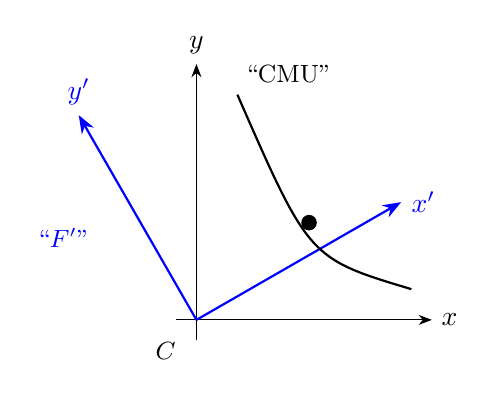
\begin{tikzpicture}[scale=1.3, >=Stealth]
  % Frame F: standard axes
  \draw[->] (-0.2,0) -- (2.3,0) node[right] {$x$};
  \draw[->] (0,-0.2) -- (0,2.5) node[above] {$y$};
  \node[font=\small] at (-0.3,-0.3) {$C$};

  % Frame F': rotated ~30 deg axes
  \draw[->, blue, thick] (0,0) -- (2.0,1.15) node[right] {$x'$};
  \draw[->, blue, thick] (0,0) -- (-1.15,2.0) node[above] {$y'$};

  % Some curved particle trajectory
  \draw[thick] (0.4,2.2) .. controls (1.1,0.6) .. (2.1,0.3);
  \filldraw (1.1,0.95) circle (2pt);

  % Labels for the two frames
  \node[font=\small] at (0.9,2.4) {``CMU''};
  \node[blue, font=\small] at (-1.3,0.8) {``$F'$''};
\end{tikzpicture}
\end{center}

The invariant distance: $x^2 + y^2 = x'^2 + y'^2$

\medskip

\begin{center}
\renewcommand{\arraystretch}{1.3}
\begin{tabular}{c|cc|cc}
  & $(x,\,y)$ & $(x',\,y')$ & & \\
  \hline
  $D$ & $0\quad 0$ & $0\quad 0$ & \multicolumn{2}{c}{} \\
  $\omega$ & $(x_0,y_0)$ & $(x'_0,y'_0)$ & & \\
  $F$ & $\cdot$ & $\cdot$ & & \\
  $C$ & $\cdot$ & $\cdot$ & & \\
\end{tabular}
\end{center}

\subsubsection*{Puzzle}

How can coordinates be both \emph{Required} and \emph{Arbitrary}?

\textbf{Answer:} Coordinates are more than just numbers!

\[
  \text{Coordinates} = \text{Numbers} + \left\{
    \begin{array}{l}
      \text{Rules to change /} \\
      \text{Prescription}
    \end{array}
  \right\} \text{ (how to transform)}
\]

``Equivalence class'' of groups of numbers related by transformations.

% ============================================================
\section*{How to Transform Between Coordinates}

Two frames $F$ and $F'$; $F'$ moves with velocity $v$ relative to $F$.
Transformation: $x(t) \longrightarrow x'(t')$.

\vspace{0.5em}

\textbf{``Time is time''} $\Rightarrow t = t'$

For $x'$, account for relative motion of $S'$:

\begin{equation*}
  x'(t) = x(t) - v_s\,t, \qquad y'=y, \quad z'=z, \quad t'=t
\end{equation*}

\subsection*{Matrix Form}

\begin{equation*}
  \begin{pmatrix} x' \\ t' \end{pmatrix}
  = \underbrace{\begin{pmatrix} 1 & v \\ 0 & 1 \end{pmatrix}}_{G(v)}
  \begin{pmatrix} x \\ t \end{pmatrix}
  = \begin{pmatrix} x + vt \\ t \end{pmatrix}
\end{equation*}

\subsubsection*{Matrix Multiplication --- Crash Course}

\begin{equation*}
  \begin{pmatrix} a_{11} & a_{12} \\ a_{21} & a_{22} \end{pmatrix}
  \begin{pmatrix} c_1 \\ c_2 \end{pmatrix}
  = \begin{pmatrix} a_{11}c_1 + a_{12}c_2 \\ a_{21}c_1 + a_{22}c_2 \end{pmatrix}
\end{equation*}

\begin{equation*}
  \begin{pmatrix} a_{11} & a_{12} \\ a_{21} & a_{22} \end{pmatrix}
  \begin{pmatrix} b_{11} & b_{12} \\ b_{21} & b_{22} \end{pmatrix}
  = \begin{pmatrix}
      a_{11}b_{11} + a_{12}b_{21} & a_{11}b_{12} + a_{12}b_{22} \\
      a_{21}b_{11} + a_{22}b_{21} & a_{21}b_{12} + a_{22}b_{22}
    \end{pmatrix}
\end{equation*}

% ============================================================
\section*{Composition of Galilean Transformations}

Two successive boosts $v_1$ then $v_2$:
\[
  x \xrightarrow{v_1} x' \xrightarrow{v_2} x''
\]

\begin{align*}
  \begin{pmatrix} x'' \\ t'' \end{pmatrix}
  &= \begin{pmatrix} 1 & v_2 \\ 0 & 1 \end{pmatrix}
     \begin{pmatrix} 1 & v_1 \\ 0 & 1 \end{pmatrix}
     \begin{pmatrix} x \\ t \end{pmatrix}
   = \begin{pmatrix} 1 & v_1 + v_2 \\ 0 & 1 \end{pmatrix}
     \begin{pmatrix} x \\ t \end{pmatrix}
\end{align*}

\[
  G(v_2)\,G(v_1) = G(v_c), \qquad v_c = v_1 + v_2
\]

\begin{tcolorbox}
  \textbf{``Galilean Transforms form a group.''} \hfill Combined velocity: $v_c = v_1 + v_2$
\end{tcolorbox}

% ============================================================
\section*{Assumption: Physics Shouldn't Depend on Coordinate Choice}

(Assertion)

Under $x' = x(t) - v_s t \;\Rightarrow\; F(x_1' - x_2') = F(x_1 - x_2)$.

\subsubsection*{What is $v'(t)$?}

\begin{align*}
  v'(t) &= \frac{dx'(t')}{dt'} = \frac{dx'(t)}{dt} = \frac{d(x(t)-v_s t)}{dt} \\[4pt]
        &= \frac{dx}{dt} - v_s\frac{dt}{dt} = v(t) - v_s
\end{align*}

\[
  v' = v(t) - v_s \qquad \Rightarrow \qquad a' = \frac{dv'}{dt} = \frac{dv}{dt} = a
\]

\[
  \boxed{\text{If } F=ma \text{ holds in one coordinate system, it holds in all.}}
\]

% ============================================================
\section*{Conservation Laws Under Galilean Boosts (HW)}

\subsubsection*{Momentum}

\begin{align*}
  \frac{d}{dt}\sum_i P_i'
    &= \sum_i m_i\,\frac{d(v(t)-v_s)}{dt}
     = \sum_i m_i\,\frac{dv_i}{dt}
     = \frac{d}{dt}\sum_i P_i
\end{align*}

$\Rightarrow$ Momentum conservation is frame-independent. $\checkmark$

\subsubsection*{Energy}

\begin{tcolorbox}
\textbf{HW:} $E$ conserved $\Rightarrow$ $P$ conserved?

\begin{align*}
  \frac{d}{dt}\sum_i E_i'
  &= \frac{d}{dt}\sum_i \frac{m_i}{2}(v_i - v_s)^2
   = \sum_i \frac{m_i}{2}\cdot 2(v_i - v_s)\frac{dv_i}{dt} \\[4pt]
  &= \sum_i\!\left(\frac{m_i}{2}\cdot 2v_i\frac{dv_i}{dt}\right) - v_s\sum_i m_i\frac{dv_i}{dt} \\[4pt]
  &= \underbrace{\frac{d}{dt}E_{tot}}_{\text{conserved}}
   - v_s\underbrace{\frac{dP_{tot}}{dt}}_{=\,0}
\end{align*}

So $\dfrac{d}{dt}E_{tot}' = \dfrac{d}{dt}E_{tot}$:
kinetic energy conservation is also frame-independent (given momentum conservation). $\checkmark$
\end{tcolorbox}

% ============================================================
\section*{Problem with Galilean Transformations}

These transformations seem very straightforward.
But (as we will see) they are \textbf{wrong\ldots}

It took \textbf{A.E.}\ (Einstein) to figure out why.

\begin{tcolorbox}
  \textbf{1\textsuperscript{st} Hint:} Maxwell's equations do \underline{NOT} satisfy the Galilean Transformation:
  \begin{itemize}
    \item Speed of light is not constant (under G.T.).
    \item $\vec{E} \leftrightarrow \vec{B}$ mix under G.T.
  \end{itemize}
\end{tcolorbox}

\end{document}
